\documentclass[a4paper, 12pt]{article}
\usepackage[table,xcdraw]{xcolor}
\usepackage[english]{babel}
\usepackage[utf8]{inputenc}
\usepackage{amsmath}
\usepackage{graphicx}
\usepackage[colorinlistoftodos]{todonotes}
\usepackage[left=2cm,right=2cm,top=2cm,bottom=2cm]{geometry}
\usepackage{comment}
\usepackage{fancyhdr}
\usepackage[font=scriptsize,labelfont=bf]{caption}
\usepackage{wrapfig}
\usepackage{afterpage}
\usepackage{titlesec}
\usepackage{setspace}
\usepackage{natbib}
\usepackage{booktabs}
\usepackage{multirow}
\usepackage{textcomp}
\usepackage{hyperref}
\hypersetup{
    colorlinks=false,
    linkcolor=.,
    filecolor=.,
    urlcolor=.,
}

\pagestyle{fancy}
\fancyhf{}
\fancyhead[R]{\includegraphics[scale = 0.05]{Logo_EPFL.png}}
\fancyhead[L]{\textcolor{gray}{ENV-540}}
\fancyfoot[R]{\textcolor{gray}{\thepage}}
\fancyfoot[L]{\textcolor{gray}{Antoine Spahr \& Joaquin Gajardo}}

\renewcommand{\headrulewidth}{0.5pt}
\renewcommand{\footrulewidth}{0.5pt}
\renewcommand{\familydefault}{\sfdefault}

\titlespacing*{\section}{0pt}{14pt}{10pt}
\titlespacing*{\subsection}{0pt}{10pt}{8pt}
\titlespacing*{\subsubsection}{0pt}{8pt}{6pt}
\titleformat{\section}
 			{\large\bfseries\sffamily}
  			{\thesection}{1em}{}
\titleformat{\subsection}
 			{\small\bfseries\sffamily}
  			{\thesubsection}{1em}{}
\titleformat{\subsubsection}
 			{\small\slshape\sffamily}
			{\thesubsubsection}{1em}{}

\begin{document}
%-------------------------------- Title ------------------------------------------
\begin{center}
    {\Large\textbf{Monitoring cocoa plantations around the Taï National Park in Ivory Coast}}
\end{center}

\begin{center}
    {\textbf{Image processing for earth observation - ENV540}}
\end{center}
Gallardo Joaquin \& Spahr Antoine \hfill {\today}
\vspace{5pt}
\hrule

%---------------------------------- Table of content -----------------------------
\pagenumbering{arabic}
\setcounter{page}{1}

%--------------------------------------- text -------------------------------------

\section{Introduction} % --> Joaquin
    % Present the scope of project : why cocoa plantation needs to be detected, what are the challenges associated (economical social and environmental). NGO reports (mighty earth), news in BBC, state of deforestation.

    %Motivation
    %Moving from national level to national park. Why Tai? last big reserve of forest, biodiversity richness (chimpanzes, etc).
    %Brief literature review
    %Goal of the report. Recognizing cocoa plantations automatically.

    Preserving forest and national parks worldwide is of utterly importance and even more so in the current climate change crisis. Forests are reserves of biodiversity and life, and perform vital roles for the planet such as storing carbon dioxide and aiding in the water and nutrient cycles \cite{grassi_key_2017, houghton_role_2015}. In Ivory Coast the forest degradation in the last decades has reached critical levels and the main direct cause is cocoa plantations as explored by Barima \textit{et al.} in their study of the Haut-Sassandra classified forest \cite{barima_cocoa_2016}. Bitty \textit{et al.} showed in their study that the presence of illegal cocoa farming in protected areas is negatively correlated with the presence of primates \cite{bitty_cocoa_2015}, highlighting the negative impact of plantations on the biodiversity. The evidence of illegal cocoa farming in Ivory Coast \cite{barima_cocoa_2016} brings to light the need of a way to monitor the national parks and nearby cocoa plantations as it can help the authorities to detect violations or risk of future violations. Multiple studies have already explored this need. In their study, Barima \textit{et al.} use a decision tree to classify Landsat images over several years to detect forest, crops and bare soil on the Haut-Sassandra protected forest \cite{barima_cocoa_2016}. Similar studies have also been conducted on the southern part of Ghana \cite{koranteng_remote_nodate} and the Metchie-Ngoum Protection Forest Reserve in the Western part of Cameroune \cite{meli_fokeng_multi-temporal_2019}. The monitoring of sustainable cacao plantations in Ivory coast has been explored by Hasan \textit{et al.} using a support vector machine (SVM) classier on high resolution Kompas-3 satellite imagery \cite{hasan_remote_2018}. Nooni \textit{et al.} used a SVM classifier to efficiently map palm oil plantation in Ghana using Landsat images \cite{nooni_support_2014}. Tutu Benefoh \textit{et al.} studied cocoa plantations in Ghana with Landsat images using supervised and unsupervised methods \cite{tutu_benefoh_assessing_2018}. Singh \textit{et al.} interestingly integrate LiDAR measurement with Landsat images to classify different forest and land use in the Phnom Kulen National Park in Cambodia. They tried three different models (SVM, random forest and an artificial neural network) and obtained good classification results \cite{singh_evaluating_2019}.
    \\
    Based on previous studies, remote sensing combined with supervised classification appears to be a powerful tool that has the potential to locate cocoa plantations in a cheap and efficient way. Even though many studies have focused on the western part of Africa to map the land use, none were found that attempt to detect cocoa plantations around the Taï National Park or any other in Ivory coast.
    \\
    \\
    That is why the goal of this study is to detect cocoa plantations with the aid of remote sensing imagery in the surroundings of the Taï National Park. The Taï is the biggest reserve of natural forest left in Ivory coast and preserving it is crucial for the conservation of the hosted biodiversity, especially chimpanzees \cite{vonk_tai_2018}. For this purpose, different supervised classification algorithms will be evaluated in order to provide a proof of concept for the monitoring of cocoa plantations around the park with free satellite imagery.

    %literatture

\section{Methods}
    \subsection{Data}

        \begin{table}[b!]
            \centering
            \caption{\textbf{Data specifications}}
            \resizebox{\textwidth}{!}{%
            \begin{tabular}{@{}cccccccccc@{}}
                \toprule
                \multirow{2}{*}{Platform} & \multirow{2}{*}{Sensor} & \multirow{2}{*}{source} & \multicolumn{2}{c}{Acquisition}                                                            & \multicolumn{3}{c}{Resolution}    & \multirow{2}{*}{CRS} & \multirow{2}{*}{Type of product} \\ \cmidrule(lr){4-8}
                                          &                         &                         & Method       & Date                                                                        & Spatial & Spectral & Radiometric  &                      &                                  \\ \midrule
                Sentinel-2                & L1C                     & EO-browser              & Sentinel-Hub & \begin{tabular}[c]{@{}c@{}}between 24.10.2019\\ and 02.12.2019\end{tabular} & 10m to 60m     & 13 bands & uint 16 bits & EPSG:4326            & Processed Level 1C                              \\ \bottomrule
                \end{tabular}%
                }
        \label{tab:data}
        \end{table}

        In order to explore the possibility of monitoring cocoa plantations, Sentinel-2 images are chosen since they are freely accessible and offers the best spatial resolution within free images (10m for the red, green, blue and near infrared [NIR] bands). The spectral resolution is rather high as well with 13 different spectral bands. Finally, Sentinel-2 provides a good coverage of the globe, which ensured that the region of interest would be accessible. It is challenging to work on forest imagery near the equator as the scene is often cloudy. That is why the focus has been given to the warm and dry season where it is easier to find a cloudless day throughout the whole region of interest. The selected images are taken on the 29.12.2018 where a clear day enables the observation of the whole park without clouds. A summary of the satellite images is provided on table \ref{tab:data}.
        \\
        \\
        The image for analysis was chosen based on the visual localization of plantations using a map of cocoa cooperatives locations \cite{Cooperatives} and Google Earth as a reference, which has a very high image resolution due to the inclusion of airborne images. Consequently, a manual ground truth labelling of plantations was perform by creating a shapefile of polygons using QGIS and visually inspecting the located plantations in Google Earth. The output of this process is presented in figure \ref{fig:overview}.

        \begin{figure}[t]
            \centering
            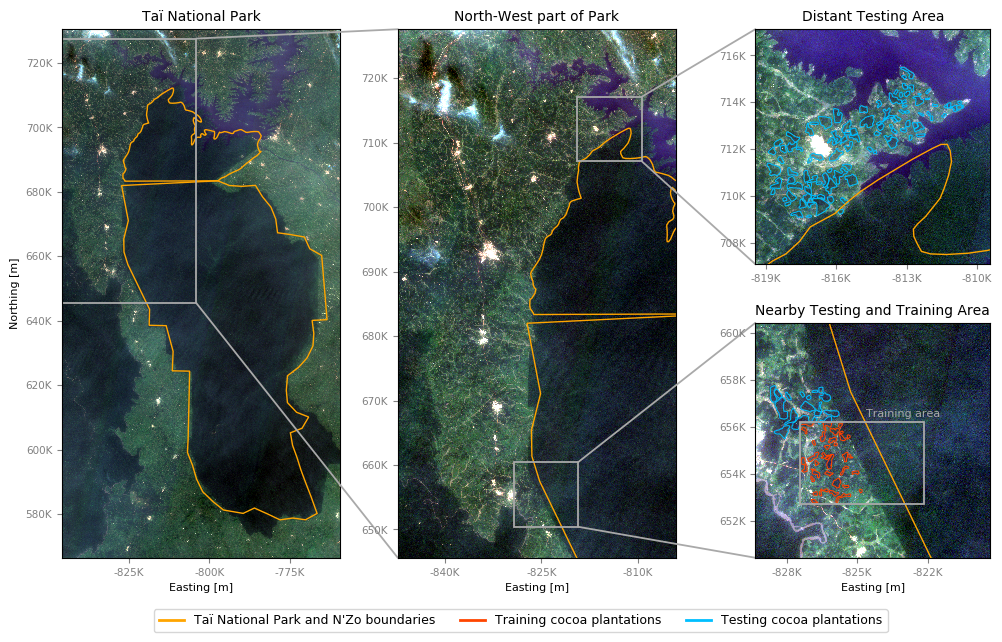
\includegraphics[width=1\textwidth]{../Figures/overview.png}
            \caption{\textbf{Data overview.} The Taï national park is situated in the South-West part of Ivory Coast close to the Liberia border. The park border is displayed in orange. North of it is the N'Zo natural reserve which is not part of the Taï national park. The boundaries shapefiles were obtained from protected planet \cite{unep-wcmc_and_iucn_protected_2019, unep-wcmc_and_iucn_protected_2019-1}. The part of the park used for training, and testing prediction (nearby and distant) are presented in the context of the whole park.}
            \label{fig:overview}
        \end{figure}

    \subsection{Model development}
        % Processing pipeline and strategy
        \begin{figure}[t]
            \centering
            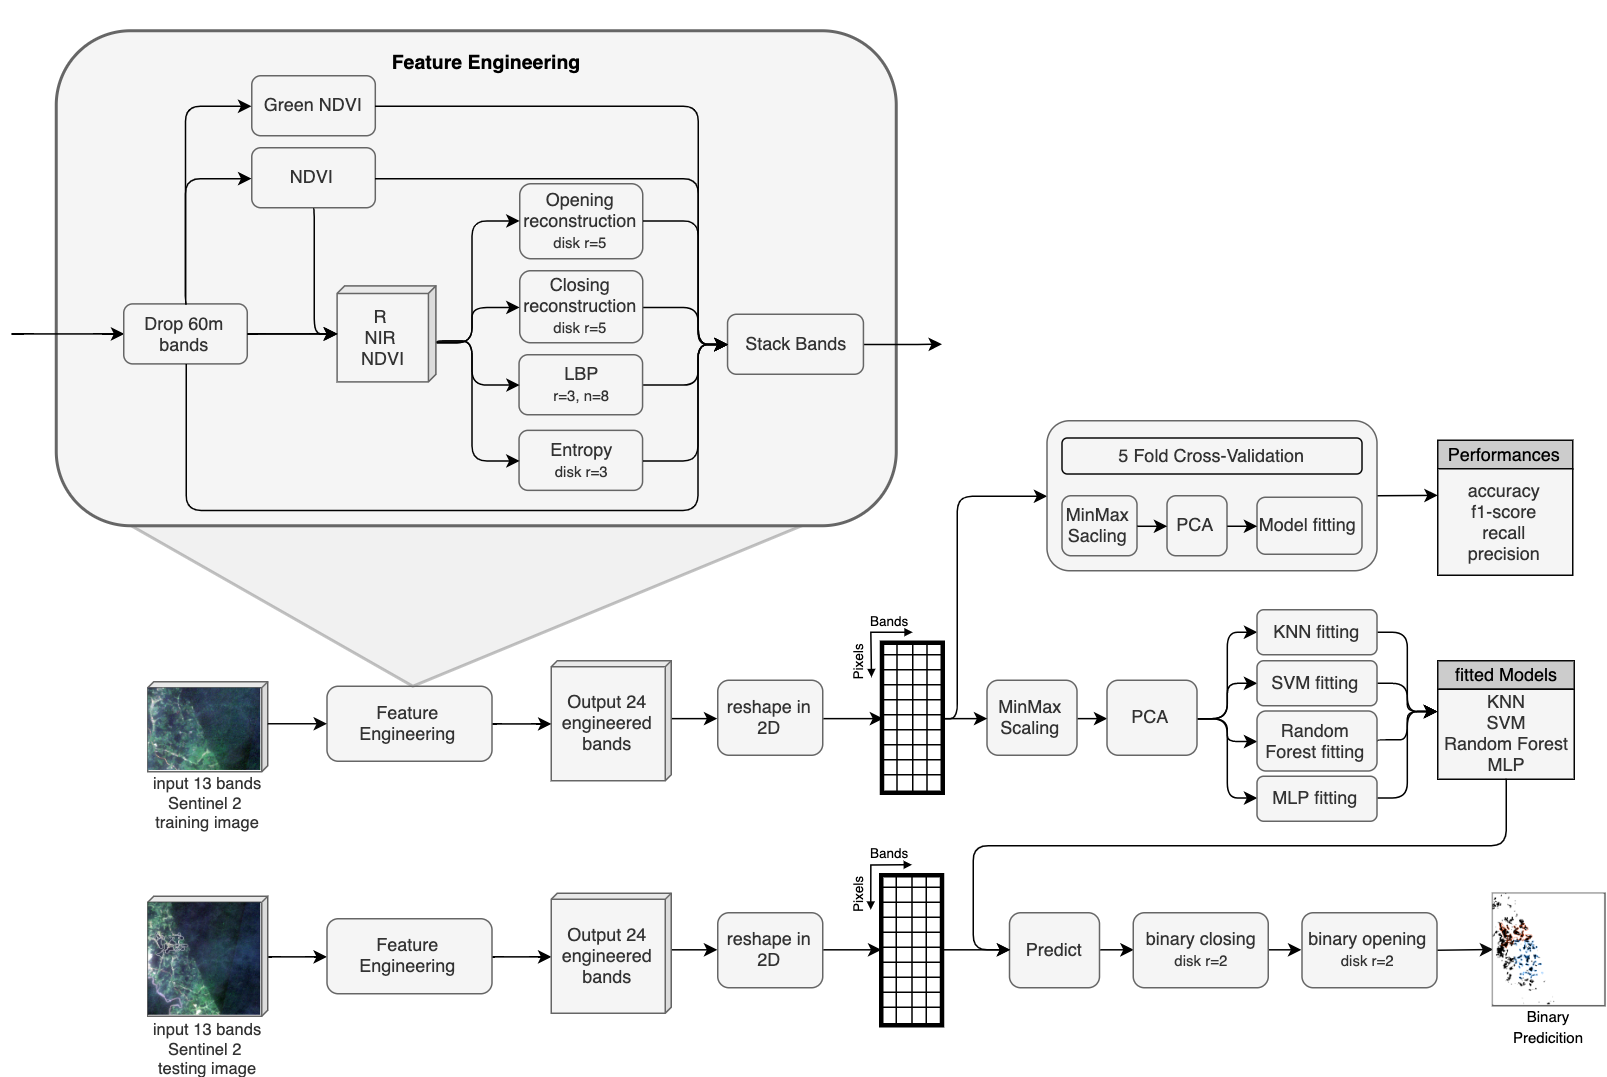
\includegraphics[width=1\textwidth]{../Figures/ProcessingDiagram.png}
            \caption{\textbf{Processing pipeline.} The flowchart presents the processing steps performed and described in the methods. The pipeline can be splited in three main group : the pre-processing, the model development and performance estimations, and the predictions.}
            \label{fig:processing}
        \end{figure}

        In order to detect the cocoa plantation from multi-spectral Sentinel-2 images, different models are developed in a supervised fashion based on the manually labeled plantations. The models construction can be separated in three phases : 1) Feature engineering, 2) Model training and 3) Prediction on new areas. The processing is visually detailed in figure \ref{fig:processing}.

        \subsubsection{Feature engineering}
            The first part of the model development consists in generating the data for the training by creating new features from the various image bands. The input image contains 13 bands (4 at a 10 meters resolution, 6 at 20 meters resolution and 3 at a 60 meters resolution). In the first place, the 60m resolution bands are dropped as their resolution is too low for the pursued application. Then the Red (R) and Near Infrared (NIR) bands are used to compute the NDVI ($= \tfrac{NIR - R}{NIR + R}$). The NDVI is a proxy for the vegetation content of a pixel as the vegetation reflects highly on NIR. Nuances in NDVI can be imputed to different types of vegetation. It may thus yield different signal between native forest and plantations. In a similar fashion the green NDVI is also computed by using the green band instead of the red and the red instead of the NIR.
            \\
            \\
            The following processing steps are applied to the R, NIR and NDVI images because of their spatial resolution of 10m and their potential discriminatory power for vegetation elements. Each of the three bands are opened by reconstruction with a disk-shaped structuring element of radius 5. This procedure aims to remove small bright elements but still keeping the structure of the original image (contrarily to a simple opening). The three bands are then closed by reconstruction with a disk-shaped structuring element of radius 5. It aims at removing small dark element of the image (dark element are low value of pixel) but also by keeping the structure of the original image. In order to extract information of the texture around a pixel (i.e. add information of neighbors), the entropy is computed over a disk of radius 2 around the given pixel. A high value indicates a rather smooth neighborhood, while a low value reflects a rather random neighborhood. In order to extract other texture information, a local binary pattern (LBP) is applied over 8 neighbors at a distance of 3 pixels from the pixel of interest. This technique should yield different values depending on the neighbors values and reflect edges, corners, etc.
            \\
            \\
            At the end of the process, 14 new features have been created which represent a total of 24 features that will be used for the training procedure.


        \subsubsection{Model training}
            The model is trained to solve the following binary classification task : classify whether a pixel close to the Taï National Park is part of a cocoa plantation or not. Therefore the models are doing pixel-wise classification. The samples are the pixels from a fully labelled area West of the park (see figure \ref{fig:overview}).\\
            The image is reshaped in a 2D array (Pixel x Bands) for the training, each pixel is a sample and each band is a feature. There are thus 24 features and 185'500 samples (350x530). The model is composed of three main blocks : a normalizer that scale all features between 0 and 1 in order to give the same power to each of them. It is followed by a PCA in order to generate decorrelated features by linearly combining the 24 original features. And finally the estimator that makes the classification. Four different estimators are explored : K-nearest-neighbors (KNN), support-vector-machine (SVM), random-forest classifier (RF) and a multilayer perceptron (MLP). The hyperparameters of the estimators are chosen as follow. For KNN five neighbors are considered to make the prediction. The SVM L2 regularization strength has been set to 1000. The RF is composed of 150 trees of maximum depth 20. The MLP contains one hidden layer of 100 neurons, and ReLU as activation function. It is trained using an Adam optimizer, a learning rate of 0.001 and maximum 200 iterations. \\
            \\
            The first step is to obtain the expected performance of each models. It is achieved by a 5-fold cross-validation. Each model is trained on 80\% of the data and tested on the 20\% of unseen, remaining data. By alternating which fold is the test set, each models is trained on five different training sets and five measures of performance are obtained. This procedure enables to obtain an estimation of performance unbiased by the choice of the train and test set, and a measure of performance with confidence intervals. Note that the normalization and PCA coefficients are estimated on the training set (excluding the test set) and they are applied on the test set to avoid introducing a bias. Indeed, this procedure avoid the training of the model to observe in advance the data it will be tested on.\\
            The performance of the models are assessed through four different metrics. The accuracy which quantifies the global correct classification. The precision which quantifies the goodness of detection (the rate of correct cacao plantation detection among the predicted cacao plantation). The recall which quantifies the rate of detection (the percentage of cacao plantation detected). And the F1-score which is the harmonic mean of the recall and the precision. A high F1-score means that the classifier detects most of the cacao plantations and predicts wrongly only a few pixel as cacao plantation. \\
            \\
            Once the performance of the models have been defined, the four models are trained with the whole training data (red polygons in figure \ref{fig:overview}).

        \subsubsection{Model predictions generalization}
            Because the models are trained on a single area where the plantation positions are known, they might learn properties specific to that area (the sampling of training sample is limited to a single zone and is thus not uniform over the area to monitor). In consequence, the models might not generalize to further areas. In order to check whether the models generalize over space, the fitted models are used to predict the pixel class of two regions outside of the training area where there are known plantations. One is a \textit{nearby prediction} and is situated just alongside the training area. The other one is a \textit{distant prediction} and is situated north of the Taï national park (see figure \ref{fig:overview}). In both cases the fitted model generates a binary image of where it thinks plantations are. Black pixels represent a plantation and are labelled with a value of 1 and white pixels are anything else and have a value of 0. Those images are usually noisy predictions as there are single pixel of predicted cocoa plantation alone and there are holes within cluster of predicted cocoa plantations. Because the plantation are usually homogeneous piece of lands bigger than 10 meters (single pixel), the model's predictions are smoothed using a morphological closing with a disk-shaped structuring element of radius 2 (disk of diameter 50 meters) to fill holes in plantation patch, followed by a morphological opening with a similar structuring element to remove small isolated plantation prediction.
            \begin{figure}[t!]
                \centering
                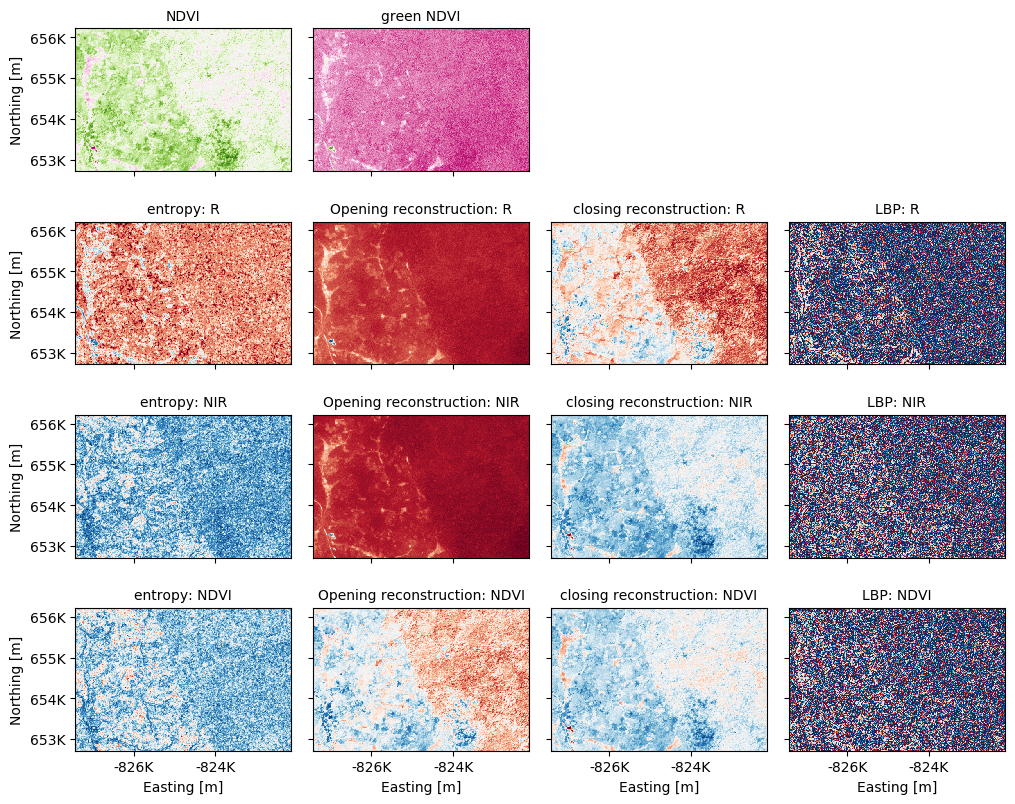
\includegraphics[width=1\textwidth]{../Figures/Feature_Engineered.png}
                \caption{\textbf{Engineered Features.} The engineered features are presented over the training area. The top row presents the NDVI and the green NDVI. A green color indicates a high positive value while pink indicate a negative value. The second, third and fourth row present the feature engineering respectively on the red (R), the near-infrared (NIR) and NDVI bands. For each of those bands red indicates a positive value and blue a negative one. For each band (R, NIR and NDVI), the entropy, the opening and closing by reconstruction, and the LBP are computed. In total, 14 new features are generated.}
                \label{fig:feature_eng}
            \end{figure}
            \\
            The quality of the detection is assessed through the recall only (\textit{i.e.} detection rate). Indeed, only some known \textit{nearby} and \textit{distant} plantations on the images have been manually labelled. The whole extent of this images have not been inspected, so the recall is preferred to overcome the effect of unlabelled plantations. The recall is calculated as the percentage of the labelled polygons that have been detected by the model (\textit{i.e.} among the labelled plantations, how much have been detected).

    \subsection{National park predictions}
        Now that the performances and predictive capabilities of the models have been explored, the best performing one can be used to predict unlabeled areas around the park. Predicting the presence of plantations over the whole park would be computationally too intensive as the park spread over around 150x50km which represents roughly 75 millions pixel to predict (10 meters resolution). Therefore only 10x10km samples of the park are predicted to explore whether the cocoa plantations violate the national park boundaries.

\section{Results}
    \subsection{Model performances}
        \subsubsection{Feature Engineering}
            The features engineered on the training image are presented on figure \ref{fig:feature_eng}. On the training image, most of the engineered features present different values between the native forest of the national park and the space used for cocoa plantations. The most discriminatives ones seems to be the closing by reconstruction on the R band and the opening by reconstruction on the NDVI. The local entropy on the NDVI images seems to extract the patches that could correspond to the cocoa plantations.

        \subsubsection{Model Performances}
            \begin{table}[b!]
                \centering
                \caption{\textbf{Models Performances} The performances of the four models estimated through 5-fold cross-validation are presented. For each model, the accuracy, f1-score, precision and recall are displayed for both the train and test folds. The performances are presented as the mean and standard deviation over the five permutations of the cross-validation. The best test performance for each metric is highlighted in pale green.}
                \resizebox{0.75\textwidth}{!}{%
                \begin{tabular}{@{}llllllllll@{}}
                    \toprule
                                                &       & \multicolumn{2}{c}{KNN}                            & \multicolumn{2}{c}{SVM}                            & \multicolumn{2}{c}{RF}                                    & \multicolumn{2}{c}{MLP}                                   \\ \midrule
                                                &       & \multicolumn{1}{c}{mean} & \multicolumn{1}{c}{std} & \multicolumn{1}{c}{mean} & \multicolumn{1}{c}{std} & \multicolumn{1}{c}{mean}        & \multicolumn{1}{c}{std} & \multicolumn{1}{c}{mean}        & \multicolumn{1}{c}{std} \\ \midrule
                                                & test  & 92.93\%                  & 0.94\%                  & 89.96\%                  & 7.68\%                  & \cellcolor[HTML]{C9E7BD}94.14\% & 0.69\%                  & \cellcolor[HTML]{C9E7BD}94.14\% & 1.31\%                  \\
                    \multirow{-2}{*}{accuracy}  & train & 95.75\%                  & 0.15\%                  & 91.27\%                  & 4.13\%                  & 99.86\%                         & 0.02\%                  & 95.46\%                         & 0.21\%                  \\
                                                & test  & 47.77\%                  & 3.46\%                  & 42.45\%                  & 17.90\%                 & 51.61\%                         & 3.09\%                  & \cellcolor[HTML]{C9E7BD}57.64\% & 4.63\%                  \\
                    \multirow{-2}{*}{f1}        & train & 68.49\%                  & 1.33\%                  & 44.24\%                  & 14.59\%                 & 99.04\%                         & 0.17\%                  & 67.30\%                         & 1.63\%                  \\
                                                & test  & 52.97\%                  & 7.99\%                  & 57.30\%                  & 23.11\%                 & \cellcolor[HTML]{C9E7BD}67.82\% & 11.47\%                 & 63.84\%                         & 12.71\%                 \\
                    \multirow{-2}{*}{precision} & train & 74.56\%                  & 1.06\%                  & 54.16\%                  & 16.25\%                 & 98.71\%                         & 0.14\%                  & 70.87\%                         & 1.76\%                  \\
                                                & test  & 44.18\%                  & 4.35\%                  & 53.57\%                  & 36.47\%                 & 43.19\%                         & 7.47\%                  & \cellcolor[HTML]{C9E7BD}54.00\% & 5.11\%                  \\
                    \multirow{-2}{*}{recall}    & train & 63.34\%                  & 1.75\%                  & 54.06\%                  & 34.96\%                 & 99.36\%                         & 0.27\%                  & 64.10\%                         & 2.22\%                  \\ \bottomrule
                \end{tabular}%
                }
                \label{tab:model_performance}
            \end{table}

            The expected performances of the four models considered are presented on table \ref{tab:model_performance} for the four metrics considered, namely the accuracy, the f1-score, the precision and the recall. Both the random forest classifier and the MLP yield the highest mean accuracy with 94.14\% \textpm \ 1.38\% (\textpm \ 2.62\%) respectively. The highest recall have been obtained with the MLP (54.00\% \textpm \ 10.22\%). However note that the KNN's recall falls in the two standard deviation range of the MLP's one. They are thus not as different as they look like due to the high standard deviation. The model displaying the highest precision is the random forest classifier, but again with a high standard deviation. Finally the f1-score is higher for the MLP (57.64\% \textpm \ 9.06\%). \\
            The random forest classifier presents some good performances on the test set, but those are really different from the train performances. This fact indicates the presence of overfitting : the model has become to specific to the training data and has thus trouble to generalize. On the other hand, the three others models show a lesser overfitting effect. \\
            Globally the accuracy is much higher than the recall, precision and f1-score. This is likely due to the imbalance of the data-set. Indeed there are more non-plantation pixels than plantation pixels. In consequence, if the models has a poor detection rate (low detection of plantation) it would still reach a high accuracy. In addition, manually labelling the plantations is likely to have introduce wrong labeling : some plantation pixels may have been omitted and some non-plantation pixels may be labeled as plantation. In consequence, the models may predict correctly those few wrongly labeled pixels but this good behavior will not be reflected in the scores. Therefore, they must be analyzed with caution.

        \subsubsection{Model Generalization}

            \begin{figure}[t!]
                \centering
                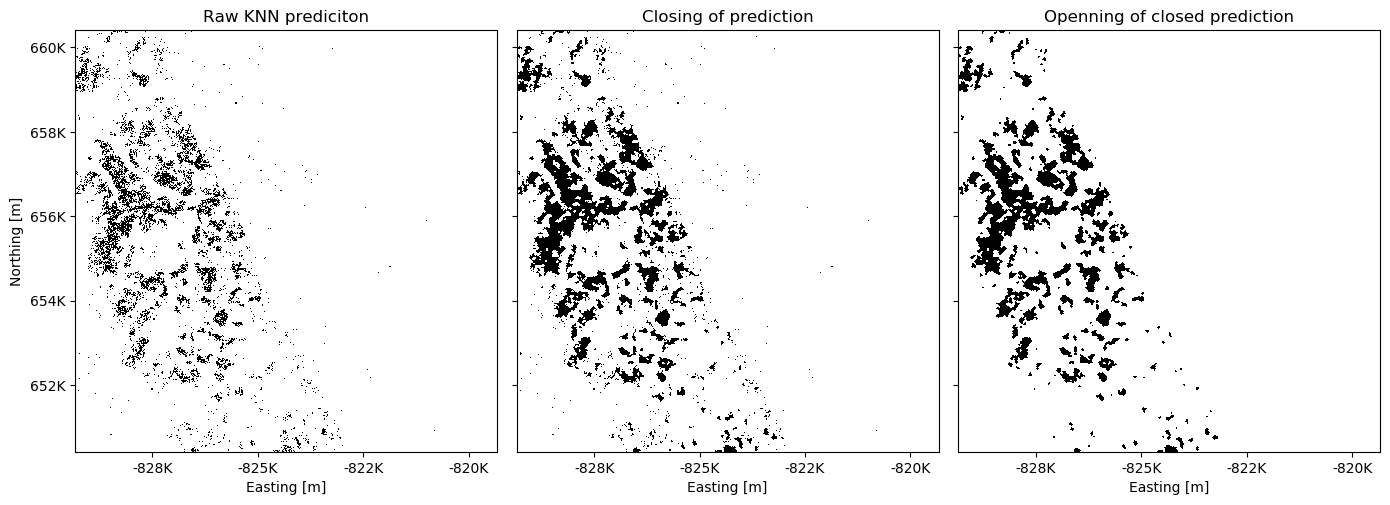
\includegraphics[width=1\textwidth]{../Figures/PostProcessing_example.png}
                \caption{\textbf{Morphological post-processing.} On the left is shown the raw prediction of the model (here the one from KNN on the nearby image). In the middle is shown the intermediate closed images to remove the 'salt' noise. On the right is shown the final post-processed image after subsequent opening to remove the 'pepper' noise.}
                \label{fig:postprocessing}
            \end{figure}

            \afterpage{%
                \begin{figure}[t!]
                    \centering
                    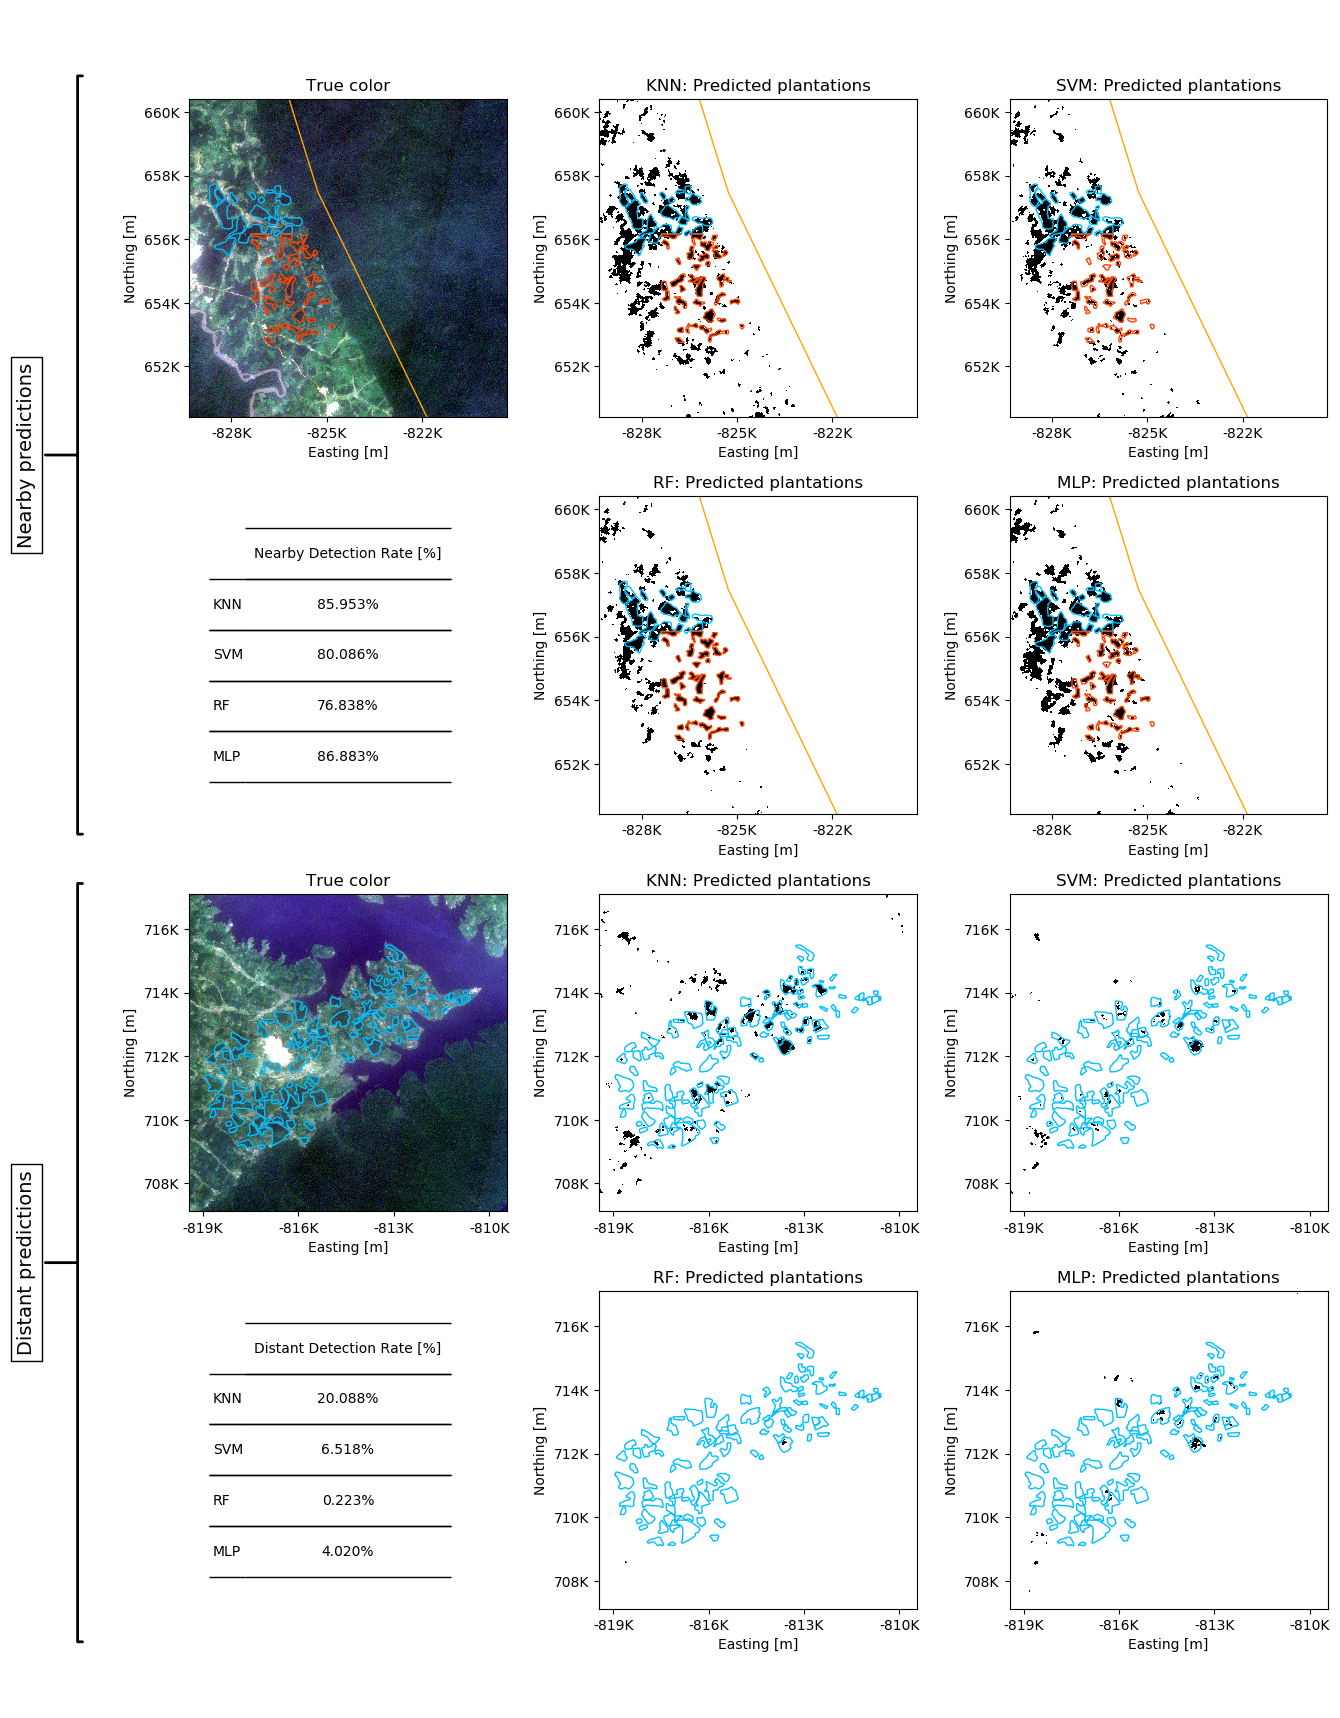
\includegraphics[width=1\textwidth]{../Figures/Tai_testing_prediction.png}
                    \caption{\textbf{Test predictions.} The prediction of the nearby (top) and distant areas (bottom) by the four models are presented. The national park boundary is displayed in orange, the training plantation are presented in red while the control (test) plantations are highlighted in blue. Those test plantation enables to assess whether the models can generalize over space. Each of the predictions presented have been post-processed with a morphological closing followed by an opening. The true color composition is also presented on the left to provide the context of the image. The boundaries shapefiles were obtained from protected planet website \cite{unep-wcmc_and_iucn_protected_2019, unep-wcmc_and_iucn_protected_2019-1}}
                    \label{fig:test_results}
                \end{figure}
                \clearpage
            }

            \afterpage{%
                \begin{figure}[t!]
                    \centering
                    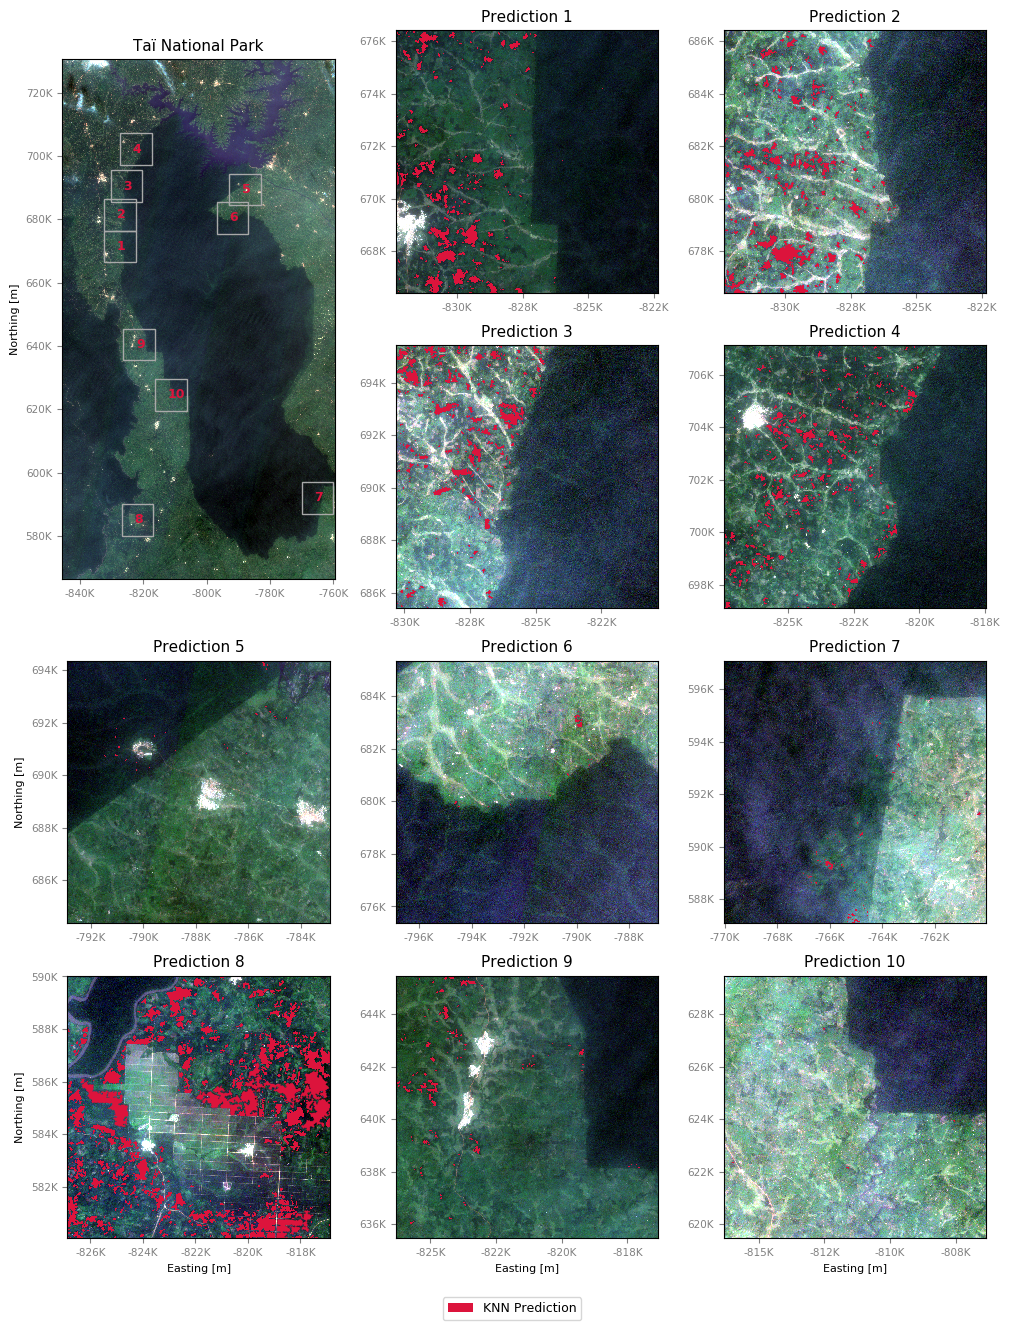
\includegraphics[width=1\textwidth]{../Figures/predictions.png}
                    \caption{\textbf{Taï national park predictions.} The top left global view presents the monitored area. The number inside the area correspond to the number on the titles of the other images. The places have been selected by hand where interesting elements seemed to be present. The red patches represent the prediction made by the KNN model. The boundaries shapefiles were obtained from protected planet \cite{unep-wcmc_and_iucn_protected_2019, unep-wcmc_and_iucn_protected_2019-1}}
                    \label{fig:prediction}
                \end{figure}
                \clearpage
            }

            The generalization over space is assessed qualitatively by visually controlling if the models predictions away from the training area detect know plantations and quantitatively by computing the recall. For this task, the model's predictions are post-processed with a morphological closing and opening. The effect of this post processing is presented on figure \ref{fig:postprocessing} for the KNN prediction on the \textit{nearby} area. The left image shows the raw KNN prediction. Main area of predicted plantations filled with 'salt' noise (\textit{i.e.} presence of white pixels within the black areas) can be observed. In addition single black pixels are also present in white area ('pepper' noise). The middle image presents the closed prediction, and shows that the 'salt' noise has been efficiently removed and the predicted areas are now uniform to patches. The image on the right presents the post-processed image after the subsequent opening. Only the main detected objects remains (larger than a disk of 50 meters radius) and the 'pepper' noise has been successfully removed.
            \\
            Two areas are used to test the models : a \textit{nearby} area around the training area and a \textit{distant} area on the north of the park (around 60km north of the training area. See figure \ref{fig:overview}). The results of the four models on both areas are presented on figure \ref{fig:test_results}. The detection rates for each model can be found on the tables of the same figure.
            \\
            The \textit{nearby} predictions of the four models yield satisfying detection of the few known plantations (blue ones). More precisely, the SVM did not detect some training plantation (red), and present thus a higher qualitative false negative rate. Oppositely, the RF classifier shows a perfect detection of the training plantations, and a still good \textit{nearby} detection but with the lowest detection rate of the four models (76.838\%). The perfect detection of the training plantations by the RF is a sign of potential overfitting. The MLP has the highest detection rate (86.883\%) and appears to provide a slightly better detection of plantations as there are (qualitatively) less false negative detection in the training area and in the testing plantation (\textit{less white in the polygons}). Finally, KNN seems to qualitatively yield the best detection results (with the post-processing). Indeed, almost all the training plantations have been detected (with some false positive), and the testing plantations are well detected (detection rate of 85.953\%).
            \\
            The four models detect less \textit{distant} plantations as presented on the bottom part of figure \ref{fig:test_results} and the detection is sparser. More precisely, the RF detected almost no plantations (0.2230\%), it thus further highlights the presence of overfitting of this model. Conversely, the MLP does not provide a good detection as, visually, only a few small patches are detected and the detection rate is rather low (4.020\%). Similarly, SVM provides also a low detection rate (6.518\%). KNN appears to be the best model of the four to detect plantations further away, as the detection is way higher (20.088\%) and visually most satisfying.
            \\
            Therefore KNN appears to be the best model of the four which is a different conclusion than from the cross-validation performances (table \ref{tab:model_performance}). This discrepancy may be due to the morphological post-processing that favor KNN in a stronger fashion. The raw predictions may have a lot of noise, thus reducing the performances reported by the cross-validation. The morphological operation that removes this noise is likely improving the classification results. In any case, it can be noted that KNN is the most reliable model for monitoring plantations that are far away from the training area.

    \subsection{National park predictions}
        The KNN model have been used to make some predictions at ten 10x10km places around the park. The results and locations of those places are presented on figure \ref{fig:prediction}. The results from figure \ref{fig:test_results} suggest that prediction further away from the training area might miss some plantations. This effect should be considered when interpreting them. Predictions 1, 2 and 3 are closer to the training area and are supposed to be more trustworthy. Globally KNN has detected multiple plantations on those images, especially the number 1, 2, 3, 4 and 8. The detection do not appear to be present within the park (here considered as the dark green area). Only prediction 5 and 7 present some small detection inside the dark green area. In the image 5, the detection gathered around a building structure. On image 7, the detection seems to be present on a brighter region of the park.

\section{Discussion}
    % feature engineering goodness and improvement
    The engineered features yields results that seems to discriminate the plantations from the rest. The goal of those features (expect the NDVIs) is to introduce local information about the neighboring pixels as the arrangement of the pixels carry meaningful information. Even though the engineered features seems relevant for the task, many other alternatives can be imagined and may likely improve the models performances.
    \\
    \\
    % performances on training
    The four models built on the training area yield good classification accuracies but the recall is lower, meaning that the models detect less of the plantations. This is likely due to the presence of 'salt' noise within patches (as in figure \ref{fig:postprocessing}). A possible source could be that what has been labeled as patch may contain pixels that may not exactly be plantations and are therefore not classified as such. Note that the models performances are computed on the raw prediction (without the morphological post-processing). Therefore the performances presented in table \ref{tab:model_performance} are likely underestimated values. Additionally, the manual labelling performed may have introduced wrongly labelled pixel in the data-set due to human error and approximate regions drawing. Moreover, the labelling from Google Earth images may suffer from temporal gap : it is not ensured that a plantation on Google Earth is already present on the Sentinel images of the 29.12.2018. In consequence, some prediction may thus be meaningful but considered as wrong reducing the performances measured by cross-validation.
    \\
    \\
    In addition, it seems that the RF classifier is overfitting as the train scores are clearly larger that the test ones. The classifier has become too specific to the training set and has trouble to generalize. This is confirmed by the testing prediction in which the RF has in both the \textit{nearby} and \textit{distant} the lowest detection rate. In the \textit{distant} case, the RF detects barely nothing. The models parameters should thus be fined tuned to reduce the overfitting effect. The amount of trees and their maximum depth could be reduced, but this could hinder the power of the model; alternatively, more features could be computed and data augmentation could be performed to enlarge the data-set and thus try to avoid overfitting.
    \\
    \\
    Based on the \textit{distant} testing, KNN appears to be the best model. However, only a single distant location with plantations have been found, labelled and used for testing. In order to better grasp the space generalization, other \textit{distant} locations with plantations should be tested as well. Indeed the image used for testing has some elements (a water body and a city) that may influence the models capabilities. The presence of water can change the atmospheric humidity, or reflect the light in a different fashion. Those small changes can change what is measured by the remote sensors and the models will be presented with an altered signal for the same object type that could lead to misclassification.
    \\
    \\
    Another dimension that has not been explored in this study is the generalization over time. Indeed, the whole work has been performed on cloudless images of the 29.12.2018 since the goal is mainly to provide a proof of concept rather than an end-product. In consequence, the models developed here may not be applicable for other dates, when the seasons may change the vegetation characteristics. If an actual detector is to be developed, the trained model should be able to generalize over space and time. To achieve this stability, the models should be trained simultaneously on different areas around the park at different dates and seasons.

\section{Conclusion}
    The present work aims to explore the use of supervised machine learning algorithms with free satellite imagery for detecting cocoa plantations in the Taï National Park of Ivory Coast. Sentinel-2 images of a single date were used throughout the project and KNN, SVM, RF and MLP algorithms were evaluated for a binary classification task on these images. Manual labelling of plantations was done in two locations around the park to provide training and testing examples. Image processing techniques were applied to perform feature engineering, that included the computation of vegetation indexes, such as NDVI and green NDVI, and texture indexes such as the entropy and LBP. Morphological operators such as opening and closing by reconstruction were also used for feature engineering and image post-processing.\\
    The results obtained show that all algorithms have a good capacity (above 75\% of detection rate) for predicting plantations that are nearby the training area, with only RF showing clear signs of overfitting. However, the algorithms show a very poor performance when tested on a distant area with plantations, with only KNN showing a detection rate over 20\%. This results prove that it is possible to detect plantations with free satellite imagery within an acceptable accuracy, provided that they are close to the original ones.\\
    Overfitting might be the obvious reason of the poor results when evaluating on distant plantations. Therefore measures like tuning the hyperparameters of the models and the computation of other relevant features could be done. Likewise, enlarging the data-set with labelled examples of other dates and locations would be advisable. Additionally, the evaluation of stronger models such as neural networks deeper than the MLP would be an interesting option.\\
    Overall, the results are promising even when used for locating plantations around the park and they prove the viability of the approach selected for the task. Nevertheless, further work is needed to improve its reliability for generalization, before being able to trust the trained models to monitor the full extension of the park and others around the country.

\newpage
\section*{Ressources}
The code used in this study is available on github at :  \url{https://github.com/antoine-spahr/Cocoa_plantations_detection}.

\footnotesize
\bibliographystyle{unsrt}
\bibliography{references}

\end{document}
